% (find-LATEX "2021-1-C2-int-subst.tex")
% (defun c () (interactive) (find-LATEXsh "lualatex -record 2021-1-C2-int-subst.tex" :end))
% (defun C () (interactive) (find-LATEXsh "lualatex 2021-1-C2-int-subst.tex" "Success!!!"))
% (defun D () (interactive) (find-pdf-page      "~/LATEX/2021-1-C2-int-subst.pdf"))
% (defun d () (interactive) (find-pdftools-page "~/LATEX/2021-1-C2-int-subst.pdf"))
% (defun e () (interactive) (find-LATEX "2021-1-C2-int-subst.tex"))
% (defun o () (interactive) (find-LATEX "2021-1-C2-int-subst.tex"))
% (defun u () (interactive) (find-latex-upload-links "2021-1-C2-int-subst"))
% (defun v () (interactive) (find-2a '(e) '(d)))
% (defun d0 () (interactive) (find-ebuffer "2021-1-C2-int-subst.pdf"))
% (defun cv () (interactive) (C) (ee-kill-this-buffer) (v) (g))
%          (code-eec-LATEX "2021-1-C2-int-subst")
% (find-pdf-page   "~/LATEX/2021-1-C2-int-subst.pdf")
% (find-sh0 "cp -v  ~/LATEX/2021-1-C2-int-subst.pdf /tmp/")
% (find-sh0 "cp -v  ~/LATEX/2021-1-C2-int-subst.pdf /tmp/pen/")
%     (find-xournalpp "/tmp/2021-1-C2-int-subst.pdf")
%     (find-xournalpp "/tmp/2021-1-C2-int-subst.pdf")
%   file:///home/edrx/LATEX/2021-1-C2-int-subst.pdf
%               file:///tmp/2021-1-C2-int-subst.pdf
%           file:///tmp/pen/2021-1-C2-int-subst.pdf
% http://angg.twu.net/LATEX/2021-1-C2-int-subst.pdf
% (find-LATEX "2019.mk")
% (find-CN-aula-links "2021-1-C2-int-subst" "2" "c2m211is" "c2is")
%
% Video:
% (find-ssr-links "c2m211is" "2021-1-C2-int-subst" "3lSrJ6sCWJI")
% (code-video     "c2m211isvideo" "$S/http/angg.twu.net/eev-videos/2021-1-C2-int-subst.mp4")
% (find-c2m211isvideo  "0:00")
% (find-c2m211isvideo  "6:00" "a obrigação de dizer: eu não entendi esse passo")
% (find-c2m211isvideo "11:12" "Então dá pra acreditar nesse TFC2 daqui")
% (find-c2m211isvideo "11:22" "Eu tou definindo uma coisa chamada [S2]")
% (find-c2m211isvideo "12:20" "e essa parte de cima eu vou chamar de a hipótese")
% (find-c2m211isvideo "14:03" "se a gente substituir o f minúsculo")
% (find-c2m211isvideo "14:30" "f(c+d) viraria")
% (find-c2m211isvideo "15:02" "que lembrem, contém uma hipótese e 3 '='s")
% (find-c2m211isvideo "15:10" "vira uma coisa que tem o mesmo formato")

% «.defs»		(to "defs")
% «.subst-defs»		(to "subst-defs")
% «.title»		(to "title")
% «.intro»		(to "intro")
% «.intro-2»		(to "intro-2")
% «.intro-3»		(to "intro-3")
% «.intro-4»		(to "intro-4")
% «.exemplo-contas»	(to "exemplo-contas")
% «.exemplo-contas-2»	(to "exemplo-contas-2")
% «.subst-int-def»	(to "subst-int-def")
% «.so-alguns-simbolos»	(to "so-alguns-simbolos")
% «.hip-triv-true»	(to "hip-triv-true")
% «.exercicio-1»	(to "exercicio-1")
% «.esquerda»		(to "esquerda")
% «.hipotese»		(to "hipotese")
% «.encontre-a-subst»	(to "encontre-a-subst")
% «.exercicio-2»	(to "exercicio-2")
% «.exercicio-2-cont»	(to "exercicio-2-cont")
% «.gambiarras-2»	(to "gambiarras-2")
% «.gambiarras-3»	(to "gambiarras-3")
% «.exercicio-5»	(to "exercicio-5")
%
% «.djvuize»	(to "djvuize")

\documentclass[oneside,12pt]{article}
\usepackage[colorlinks,citecolor=DarkRed,urlcolor=DarkRed]{hyperref} % (find-es "tex" "hyperref")
\usepackage{amsmath}
\usepackage{amsfonts}
\usepackage{amssymb}
\usepackage{pict2e}
\usepackage[x11names,svgnames]{xcolor} % (find-es "tex" "xcolor")
\usepackage{colorweb}                  % (find-es "tex" "colorweb")
%\usepackage{tikz}
%
% (find-dn6 "preamble6.lua" "preamble0")
%\usepackage{proof}   % For derivation trees ("%:" lines)
%\input diagxy        % For 2D diagrams ("%D" lines)
%\xyoption{curve}     % For the ".curve=" feature in 2D diagrams
%
\usepackage{edrx21}               % (find-LATEX "edrx21.sty")
\input edrxaccents.tex            % (find-LATEX "edrxaccents.tex")
\input edrx21chars.tex            % (find-LATEX "edrx21chars.tex")
\input edrxheadfoot.tex           % (find-LATEX "edrxheadfoot.tex")
\input edrxgac2.tex               % (find-LATEX "edrxgac2.tex")
%
%\usepackage[backend=biber,
%   style=alphabetic]{biblatex}            % (find-es "tex" "biber")
%\addbibresource{catsem-slides.bib}        % (find-LATEX "catsem-slides.bib")
%
% (find-es "tex" "geometry")
\usepackage[a6paper, landscape,
            top=1.5cm, bottom=.25cm, left=1cm, right=1cm, includefoot
           ]{geometry}
%
\begin{document}

%\catcode`\^^J=10
%\directlua{dofile "dednat6load.lua"}  % (find-LATEX "dednat6load.lua")

% %L dofile "edrxtikz.lua"  -- (find-LATEX "edrxtikz.lua")
% %L dofile "edrxpict.lua"  -- (find-LATEX "edrxpict.lua")
% \pu

% «defs»  (to ".defs")
% (find-LATEX "edrx15.sty" "colors-2019")
%\long\def\ColorRed   #1{{\color{Red1}#1}}
%\long\def\ColorViolet#1{{\color{MagentaVioletLight}#1}}
%\long\def\ColorViolet#1{{\color{Violet!50!black}#1}}
%\long\def\ColorGreen #1{{\color{SpringDarkHard}#1}}
%\long\def\ColorGreen #1{{\color{SpringGreenDark}#1}}
%\long\def\ColorGreen #1{{\color{SpringGreen4}#1}}
%\long\def\ColorGray  #1{{\color{GrayLight}#1}}
%\long\def\ColorGray  #1{{\color{black!30!white}#1}}
%\long\def\ColorBrown #1{{\color{Brown}#1}}
%\long\def\ColorBrown #1{{\color{brown}#1}}
%\long\def\ColorOrange#1{{\color{orange}#1}}
%
%\long\def\ColorShort #1{{\color{SpringGreen4}#1}}
%\long\def\ColorLong  #1{{\color{Red1}#1}}
%
%\def\frown{\ensuremath{{=}{(}}}
%\def\True {\mathbf{V}}
%\def\False{\mathbf{F}}
%\def\D    {\displaystyle}

% (find-LATEX "2017planar-has-defs.tex" "sa-and-ga")
\def\sa#1#2{\expandafter\def\csname myarg#1\endcsname{#2}}
\def\ga#1{\csname myarg#1\endcsname}

\def\Rd#1{{\ColorRed{#1}}}
\def\Rdq {{\ColorRed{?}}}

\def\drafturl{http://angg.twu.net/LATEX/2021-1-C2.pdf}
\def\drafturl{http://angg.twu.net/2021.1-C2.html}
\def\draftfooter{\tiny \href{\drafturl}{\jobname{}} \ColorBrown{\shorttoday{} \hours}}




% «subst-defs»  (to ".subst-defs")
% (find-LATEX "2020-1-C2-TFC2-2.tex" "subst-defs")

\def\pfo#1{\ensuremath{\mathsf{[#1]}}}
\def\veq{\rotatebox{90}{$=$}}
\def\Rd{\ColorRed}
\def\D{\displaystyle}

% Difference with mathstrut
\def\Difms #1#2#3{\left. \mathstrut #3 \right|_{s=#1}^{s=#2}}
\def\Difmu #1#2#3{\left. \mathstrut #3 \right|_{u=#1}^{u=#2}}
\def\Difmx #1#2#3{\left. \mathstrut #3 \right|_{x=#1}^{x=#2}}
\def\Difmth#1#2#3{\left. \mathstrut #3 \right|_{θ=#1}^{θ=#2}}

\def\iequationbox#1#2{
    \left(
    \begin{array}{rcl}
    \D{ #1 } &=& \D{ #2 } \\
    \end{array}
    \right)
  }
\def\isubstbox#1#2#3#4#5{{
    \def\veq{\rotatebox{90}{$=$}}
    \def\ph{\phantom}
    \left(
    \begin{array}{rcl}
    \D{ #1 } &=& \D{ #2 } \\
    {\veq#3} \\
    \D{ #4 } &=& \D{ #5 } \\
    \end{array}
    \right)
  }}
\def\isubstboxT#1#2#3#4#5#6{{
    \def\veq{\rotatebox{90}{$=$}}
    \def\ph{\phantom}
    \left(
    \begin{array}{rcl}
    \multicolumn{3}{l}{\text{#6}} \\%[5pt]
    \D{ #1 } &=& \D{ #2 } \\
    {\veq#3} \\
    \D{ #4 } &=& \D{ #5 } \\
    \end{array}
    \right)
  }}
\def\isubstboxTT#1#2#3#4#5#6#7{{
    \def\veq{\rotatebox{90}{$=$}}
    \def\ph{\phantom}
    \left(
    \begin{array}{rcl}
    \multicolumn{3}{l}{\text{#6}} \\%[5pt]
    \D{ #1 } &=& \D{ #2 } \\
    {\veq#3} \\
    \D{ #4 } &=& \D{ #5 } \\
    \multicolumn{3}{l}{\text{#7}} \\%[5pt]
    \end{array}
    \right)
  }}

% Definição das fórmulas para integração por substituição.
% Algumas são pmatrizes 3x3 usando isubstbox.

\def\TFCtwo{
  \iequationbox {\Intx{a}{b}{F'(x)}}
                {\Difmx{a}{b}{F(x)}}
}
\def\TFCtwoI{
  \iequationbox {\intx{F'(x)}}
                {F(x)}
}

\def\Sone{
  \isubstbox
    {\Difmx{a}{b}{f(g(x))}}  {\Intx{a}{b}{f'(g(x))g'(x)}}
    {\ph{mmm}}
    {\Difmu{g(a)}{g(b)}{f(u)}} {\Intu{g(a)}{g(b)}{f'(u)}}
}
\def\SoneI{
  \isubstbox
    {f(g(x))} {\intx{f'(g(x))g'(x)}}
    {\ph{m}}
    {f(u)}    {\intu{f'(u)}}
}

\def\Stwo{
  \isubstboxT
    {\Difmx{a}{b}{F(g(x))}}   {\Intx{a}{b}{f(g(x))g'(x)}}
    {\ph{mmm}}
    {\Difmu{g(a)}{g(b)}{F(u)}}  {\Intu{g(a)}{g(b)}{f(u)}}
    {Se $F'(u)=f(u)$ então:}
}
\def\StwoI{
  \isubstboxT
    {F(g(x))}  {\intx{f(g(x))g'(x)}}
    {\ph{m}}
    {F(u)}     {\intu{f(u)}}
    {Se $F'(u)=f(u)$ então:}
}
\def\StwoI{
  \isubstboxTT
    {F(g(x))}  {\intx{f(g(x))g'(x)}}
    {\ph{m}}
    {F(u)}     {\intu{f(u)}}
    {Se $F'(u)=f(u)$ então:}
    {Obs: $u=g(x)$.}
}

\def\Sthree{
  \iequationbox {\Intx{a}{b}{f(g(x))g'(x)}}
                {\Intu{g(a)}{g(b)}{f(u)}}
}
\def\SthreeI{
  \iequationbox {\intx{f(g(x))g'(x)}}
                {\intu{f(u)}
                 \qquad [u=g(x)]
                }
  % [u=g(x)]
}

\def\Sthree{
  \pmat{
    \D \Intx{a}{b}{f(g(x))g'(x)} \\
    \veq \\
    \D \Intu{g(a)}{g(b)}{f(u)}
  }}

\def\SthreeI{
  \pmat{
    \D \intx{f(g(x))g'(x)} \\
       \veq \\
    \D \intu{f(u)} \\
    \text{Obs: $u=g(x)$.} \\
  }}



\def\Subst#1{\bmat{#1}}



%  _____ _ _   _                               
% |_   _(_) |_| | ___   _ __   __ _  __ _  ___ 
%   | | | | __| |/ _ \ | '_ \ / _` |/ _` |/ _ \
%   | | | | |_| |  __/ | |_) | (_| | (_| |  __/
%   |_| |_|\__|_|\___| | .__/ \__,_|\__, |\___|
%                      |_|          |___/      
%
% «title»  (to ".title")
% (c2m211isp 1 "title")
% (c2m211isa   "title")

\thispagestyle{empty}

\begin{center}

\vspace*{1.2cm}

{\bf \Large Cálculo 2 - 2021.1}

\bsk

Aula 21: integração por substituição

\bsk

Eduardo Ochs - RCN/PURO/UFF

\url{http://angg.twu.net/2021.1-C2.html}

\end{center}

\newpage

% «intro»  (to ".intro")
% (c2m211isp 2 "intro")
% (c2m211isa   "intro")

{\bf Introdução}

\ssk

No último PDF, que era sobre os dois TFCs,

nós começamos a ver que podíamos calcular integrais

sem os limites de integração e colocá-los só no final,

e vimos que várias das nossas fórmulas de integração

vão tem uma versão pra integrais definidas e uma

outra pra integrais indefinidas...

Por exemplo:

\def\Ps  #1{\left( #1 \right) }
\def\ps  #1{     ( #1       ) }
\def\nops#1{       #1         }
\def\righte{\quad\text{e}}

$$
\begin{array}{rc}
  \text{TFC2:}
    & \Ps{\begin{array}{rcl}
              \D \Intx{a}{b}{F'(x)} &=& \difx{a}{b}{F(x)}
           \end{array}}
  \\[15pt]
  \text{TFC2I:}
    & \Ps{\begin{array}{rcl}
              \D \intx      {F'(x)} &=&            {F(x)}
           \end{array}}
\end{array}
$$


\newpage

% «intro-2»  (to ".intro-2")
% (c2m211isp 3 "intro-2")
% (c2m211isa    "intro-2")

{\bf Introdução (2)}

\ssk

Lembre que nós às vezes dávamos nomes como

[TFC2] e [TFC2I] pras nossas fórmulas, pra

ficar mais fácil usá-las em subtituições...

Então:


$$
\begin{array}{rcc}
  \text{[TFC2]}
    & =
    & \Ps{\begin{array}{rcl}
              \D \Intx{a}{b}{F'(x)} &=& \difx{a}{b}{F(x)}
           \end{array}}
  \\[15pt]
  \text{[TFC2I]}
    & =
    & \Ps{\begin{array}{rcl}
              \D \intx      {F'(x)} &=&            {F(x)}
           \end{array}}
\end{array}
$$


\newpage

% «intro-3»  (to ".intro-3")
% (c2m211isp 4 "intro-3")
% (c2m211isa   "intro-3")

{\bf Introdução (3)}

\ssk

Uma das técnicas que vai ser mais úteis pra calcular

integrais complicadas é {\sl integração por substituição},

em que a gente inventa uma variável nova, substitui

ela de vários jeitos (!!!) na integral original, e com

isso a gente consegue transformar a integral anterior

numa outra integral mais simples, mas que é em outra

variável e tem outros limites de integração...

\msk

\newpage

% «intro-4»  (to ".intro-4")
% (c2m211isp 5 "intro-4")
% (c2m211isa   "intro-4")

{\bf Introdução (4)}

\ssk

Aqui as duas figuras à direita têm a mesma área.

A primeira corresponde a uma integral mais complicada

que a segunda, e pra passar da primeira pra segunda

a gente amassou a figura na vertical e esticou ela

na horizontal de um modo que não alterou a área dela...


% (c2m202tfcp 9 "intro")
% (c2m202tfca   "intro")

$$\begin{array}{rcl}
  \D \Intx{π/4}{π/2}{2 \sen 2x}
  &=&
  \Area\left(
  % (find-latexscan-links "C2" "20210316_sen_2")
  % (find-xpdf-page "~/LATEX/2020-2-C2/20210316_sen_2.pdf")
  \myvcenter{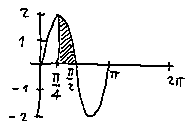
\includegraphics[height=2cm]{2020-2-C2/20210316_sen_2.pdf}}
  \right)
  \\
  \D \Intx{π/2}{π}{\sen x}
  &=&
  \Area\left(
  % (find-latexscan-links "C2" "20210316_sen_1")
  % (find-xpdf-page "~/LATEX/2020-2-C2/20210316_sen_1.pdf")
  \myvcenter{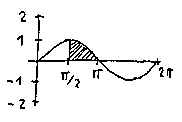
\includegraphics[height=2cm]{2020-2-C2/20210316_sen_1.pdf}}
  \right)
  \\
  \end{array}
  \\
$$

\newpage

% «exemplo-contas»  (to ".exemplo-contas")
% (c2m211isp 6 "exemplo-contas")
% (c2m211isa   "exemplo-contas")
% (c2m202isp 9 "exemplo-gamb")
% (c2m202isa   "exemplo-gamb")

{\bf Um exemplo com contas}

Isto aqui é um exemplo de como contas com integração

por substituição costumam ser feitas na prática:
%
$$\scalebox{0.95}{$
  \begin{array}{l}
  \D \intx{2 \cos(3x+4)} \\[8pt]
  = \;\; \D \intu {2 (\cos u) · \frac13}
    \\[8pt]
  = \;\; \D \frac23 \intu{\cos u} \\[8pt]
  = \;\; \D \frac23 \sen u \\[8pt]
  = \;\; \D \frac23 \sen (3x+4) \\
  \end{array}
  $}
$$

É necessário indicar em algum lugar que a relação

entre a variável nova e a antiga é esta: $u=3x+4$.

\newpage

% «exemplo-contas-2»  (to ".exemplo-contas-2")
% (c2m211isp 7 "exemplo-contas-2")
% (c2m211isa   "exemplo-contas-2")

{\bf Outro exemplo com contas}
%
\def\S{\sen x}
\def\C{\cos x}
\def\und#1#2{\underbrace{#1}_{#2}}
%
$$\begin{array}[t]{l}
  \D \intx{(\S)^5 (\C)^3} \\
  \D = \;\; \intx{(\S)^5 (\C)^2 (\C)} \\
  \D = \;\; \intx{(\und{\S}{s})^5 \und{(\C)^2}{1-s^2} \und{(\C)}{\frac{ds}{dx}}} \\
  \D = \;\; \ints{s^5 (1-s^2)} \\
  \D = \;\; \ints{s^5 - s^7} \\
  \D = \;\; \frac{s^6}{6} - \frac{s^8}{8} \\
  \D = \;\; \frac{(\S)^6}{6} - \frac{(\S)^8}{8} \\
  \end{array}
  \qquad
  \begin{array}[t]{c}
  \\ \\
    \bmat{s = \sen x \\
          \frac{ds}{dx} = \cos x \\
          \sen x = s \\
          (\cos x)^2 = 1 - s^2 \\
          \cos x \, dx = ds
    }
  \end{array}
$$

\newpage

% «subst-int-def»  (to ".subst-int-def")
% (c2m211isp 8 "subst-int-def")
% (c2m211isa   "subst-int-def")

{\bf Substituição na integral definida}

Eu vou chamar a \ColorRed{demonstração} abaixo de \pfo{S2}.

Ela é uma série de três igualdades: o `$=$' de cima,

o `$=$' de baixo, e o `$=$' da esquerda (que é um `$\,\rotl{=}$').

Eu vou chamar o ``$F'(u)=f(u)$'' de a \ColorRed{hipótese} do \pfo{S2}.

Obs: nós \ColorRed{ainda} não acreditamos nessa demonstração...

vamos verificar as igualdades dela daqui a alguns slides.
%
% (c2m202isp 3 "def-S2-S2I")
% (c2m202isa   "def-S2-S2I")
%
$$\begin{array}{rcc}
 \pfo{S2} &=& \Stwo \\
 % \\
 % \pfo{S2I} &=& \StwoI \\
 \end{array}
$$


\newpage

% «so-alguns-simbolos»  (to ".so-alguns-simbolos")
% (c2m211isp 9 "so-alguns-simbolos")
% (c2m211isa   "so-alguns-simbolos")

Lembre que dá pra substituir só alguns símbolos...

Por exemplo:
%
\def\Stwotmp{
  \isubstboxT
    {\Difmx{a}{b}{F(2x)}}   {\Intx{a}{b}{f(2x)·2}}
    {\ph{mmm}}
    {\Difmu{2a}{2b}{F(u)}}  {\Intu{2a}{2b}{f(u)}}
    {Se $F'(u)=f(u)$ então:}
}
%
$$\scalebox{0.9}{$
  \begin{array}{c}
 \pfo{S2} \;\;=\;\; \Stwo \\
 [50pt]
 \pfo{S2}[g(x):=2x] \;\;=\;\; \Stwotmp \\
 \end{array}
  $}
$$

\newpage

% «hip-triv-true»  (to ".hip-triv-true")
% (c2m211isp 10 "hip-triv-true")
% (c2m211isa    "hip-triv-true")

Também podemos substituir o $f$ por $F'$...

E aí a hipótese passa a ser ``trivialmente verdadeira'':
%
\def\Stwotmp{
  \isubstboxT
    {\Difmx{a}{b}{F(g(x))}}   {\Intx{a}{b}{F'(g(x))g'(x)}}
    {\ph{mmm}}
    {\Difmu{g(a)}{g(b)}{F(u)}}  {\Intu{g(a)}{g(b)}{F'(u)}}
    {Se $F'(u)=F'(u)$ então:}
}
%
$$\scalebox{0.9}{$
  \begin{array}{c}
  \pfo{S2} \;\;=\;\; \Stwo \\
  [50pt]
  \pfo{S2}[f(u):=F'(u)] \;\;=\;\; \Stwotmp \\
  \end{array}
  $}
$$

\newpage

% «exercicio-1»  (to ".exercicio-1")
% (c2m211isp 11 "exercicio-1")
% (c2m211isa    "exercicio-1")

{\bf Exercício 1.}

Lembre que:
%
$$\pfo{TFC2}
  \;\;=\;\;
  \Ps{
       \D \Intx{a}{b}{\ddx F(x)} \;\;=\;\; \difx{a}{b}{F(x)}
     }
$$

\msk

Calcule os resultados destas expansões:

a) $\pfo{TFC2} \bmat{F(x):=F(g(x))}$

b) $\pfo{TFC2} \bmat{x:=u} \bmat{a:=g(a) \\ b:=g(b)}$

\bsk
\bsk

...e verifique que \ColorRed{se $f(u)=F'(u)$ então}:

c) o que você obteve no (a) prova o `$=$' de cima da \pfo{S2},

d) o que você obteve no (b) prova o `$=$' de baixo da \pfo{S2},


\newpage

% «esquerda»  (to ".esquerda")
% (c2m211isp 12 "esquerda")
% (c2m211isa    "esquerda")

O `$\,\rotl{=}$' à esquerda na \pfo{S2}

é bem fácil de verificar... ó:

$$\begin{array}{rcl}
  \difx{a}{b}{F(g(x))} &=& F(g(b)) - F(g(a)) \\
                       &=& \difu{g(a)}{g(b)}{F(u)}
  \end{array}
$$

\bsk
\bsk

Se você conseguiu fazer todos os itens

do exercício 1 e conseguiu entender isso aí

então \ColorRed{agora} você entende o $\pfo{S2}$ como uma

demonstração --- você entende todas as

igualdades dele.


\newpage

% «hipotese»  (to ".hipotese")
% (c2m211isp 13 "hipotese")
% (c2m211isa    "hipotese")

{\bf Pra que serve a hipótese do \pfo{S2}?}

Ela serve pra gente lidar com `$f$'s que a gente

não sabe integrar! Por exemplo:
%
\def\Stwotmp{
  \isubstboxT
    {\Difmx{a}{b}{F(g(x))}}   {\Intx{a}{b}{\tan(g(x))\tan'(x)}}
    {\ph{mmm}}
    {\Difmu{g(a)}{g(b)}{F(u)}}  {\Intu{g(a)}{g(b)}{\tan(u)}}
    {Se $F'(u)=F'(u)$ então:}
}
%
\def\Stwotmp{
  \isubstboxT
    {\Difmx{a}{b}{F(2x)}}   {\Intx{a}{b}{\tan(2x)·2}}
    {\ph{mmm}}
    {\Difmu{g(a)}{g(b)}{F(u)}}  {\Intu{2a}{2b}{\tan(u)}}
    {\ColorRed{Se $F'(u)=\tan u$ então:}}
}
%
$$\scalebox{0.90}{$
  \begin{array}{c}
  \pfo{S2} \;\;=\;\; \Stwo \\
  [50pt]
  % \pfo{S2}[f(x):=\tan x] \;\;=\;\; \Stwotmp \\
    \pfo{S2}\bmat{f(x):=\tan x \\ g(u):=2u} \;\;=\;\; \Stwotmp \\
  \end{array}
  $}
$$

\newpage

{\bf Uma versão do \pfo{S2} para integrais indefinidas}

Compare... e repare no ``\ColorRed{Obs: $u = g(x)$}''.
%
\def\StwoItmp{
  \isubstboxTT
    {F(g(x))}  {\intx{f(g(x))g'(x)}}
    {\ph{m}}
    {F(u)}     {\intu{f(u)}}
    {Se $F'(u)=f(u)$ então:}
    {\ColorRed{Obs: $u=g(x)$.}}
}
%
$$\scalebox{0.90}{$
  \begin{array}{c}
  \pfo{S2} \;\;=\;\; \Stwo \\
  [50pt]
  \pfo{S2I} \;\;=\;\; \StwoItmp \\
  \end{array}
  $}
$$

\newpage

{\bf Versões sem a parte da esquerda}

Compare:
%
$$\scalebox{0.90}{$
  \begin{array}{c}
  \pfo{S2} \;\;=\;\; \Stwo \\
  [50pt]
  \pfo{S3} \;\;=\;\; \Sthree \\
  \end{array}
  $}
$$

\newpage

{\bf Versões sem a parte da esquerda (2)}

...e compare:
%
$$\scalebox{0.90}{$
  \begin{array}{c}
  \pfo{S2I} \;\;=\;\; \StwoI \\
  [50pt]
  \pfo{S3I} \;\;=\;\; \SthreeI \\
  \end{array}
  $}
$$

\newpage

% «encontre-a-subst»  (to ".encontre-a-subst")
% (c2m211isp 17 "encontre-a-subst")
% (c2m211isa    "encontre-a-subst")

As pessoas costumam usar variações da $\pfo{S3I}$,

geralmente sem darem um nome pra função $g(u)$...


Lembre que em vários exercícios que nós já fizemos

ficava implícito que vocês tinham que descobrir qual

era a substituição certa... por exemplo:
%
$$\begin{array}{rcl}
  \difx{4}{5}{x^2} &=& \Rdq \\[5pt]
  \Ps{\difx{a}{b}{f(x)} = f(b)-f(a)} \bmat{f(x):=\Rdq \\ a:=\Rdq \\ b:=\Rdq} &=& \Rdq
  \\[20pt]
  \Ps{\difx{a}{b}{f(x)} = f(b)-f(a)} \bmat{f(x):=x^2  \\ a:=4    \\ b:=5} &=&
  \Ps{\difx{4}{5}{x^2} = 5^2-4^2} \\
  [20pt]
  \difx{4}{5}{x^2} &=& 5^2 - 4^2 \\
  \end{array}
$$


\newpage

% «exercicio-2»  (to ".exercicio-2")
% (c2m211isp 18 "exercicio-2")
% (c2m211isa    "exercicio-2")

{\bf Exercício 2.}

Nos livros e nas notas de aula que você vai encontrar por aí

o ``\ColorRed{Obs: $u = g(x)$}'' da nossa \pfo{S3I} quase sempre aparece escrito

de (ZILHÕES DE!!!) outros jeitos, então o melhor que a gente

pode fazer é tentar encontrar as substituições que transformam

a nossa \pfo{S3I} em algo ``mais ou menos equivalente'' às

igualdades complicadas que eu mostrei no vídeo e que eu disse

que a gente iria tentar decifrar...

\msk

Nos itens a e b deste exercício você vai tentar encontrar

as substituições --- que eu vou escrever como `$[\Rdq]$' --- que

transformam a $\pfo{S3I}$ em algo ``mais ou menos equivalente''

às igualdades da direita.

\newpage

% «exercicio-2-cont»  (to ".exercicio-2-cont")
% (c2m211isp 19 "exercicio-2-cont")
% (c2m211isa    "exercicio-2-cont")

{\bf Exercício 2 (cont.)}

Encontre as substituições `$[\Rdq]$'s que façam com que:

\bsk

a) $\SthreeI [\Rdq]$ vire algo como
   $\pmat{ \D \intx{2 \cos(3x+4)} \\
           \rotl{=} \\
           \D \intu {2 (\cos u) · \frac13} \\
         }$

\msk

b) $\pfo{S3I} \, [\Rdq]$ vire algo como
   $\pmat{ \D \intx{(\S)^5 (1 - \S^2) (\C)} \\
           \rotl{=} \\
           \D \ints{s^5 (1-s^2)} \\
         }$


\newpage

{\bf Gambiarras}

Em geral é mais prático a gente usar umas gambiarras

como ``$\frac{du}{dx}dx = du$'' ao invés do método ``mais honesto''

que a gente usou no exercício 2...

\msk

Às vezes essas gambiarras vão usar uma versão disfarçada

do teorema da derivada da função inversa: $\frac{du}{dx} = \frac{1}{\frac{dx}{du}}$,

e umas outras manipulações esquisitas de `$dx$'s e `$du$'s

que só aparecem explicadas direito nos capítulos sobre

``diferenciais'' dos livros de Cálculo.

\msk

Nós vamos começar usando elas como gambiarras mesmo,

e acho que nesse semestre não vai dar pra ver como

traduzir cada uma delas pra algo formal...

\newpage

% «gambiarras-2»  (to ".gambiarras-2")
% (c2m211isp 21 "gambiarras-2")
% (c2m211isa    "gambiarras-2")

{\bf Gambiarras (2)}

Quando a gente está começando e ainda não tem prática

este modo de por anotações embaixo de chaves ajuda muito:
%
$$%\begin{array}{c}
  \D \int  (\und{\S}{s})^5
           (1 - (\und{\S}{s})^2)
           \und{
           \und{(\C)}{\frac{ds}{dx}} \, dx
           }{ds}
            \\
  % \rotl{=} \\
  \;\; = \;\;
  \D \ints{s^5 (1-s^2)} \\
  % \end{array}
$$

Quando a gente já tem mais prática acaba sendo melhor

pôr todas as anotações dentro de caixinhas --- por exemplo:

$$\bmat{
  \sen x = s \\
  \frac{ds}{dx} = \frac{d}{dx} \sen x = \cos x \\
  \cos x \, dx = ds \\
  }
$$


\newpage

% «gambiarras-3»  (to ".gambiarras-3")
% (c2m211isp 22 "gambiarras-3")
% (c2m211isa    "gambiarras-3")

{\bf Gambiarras (3)}

Essas caixinhas, como
%
$$\bmat{
  \sen x = s \\
  \frac{ds}{dx} = \frac{d}{dx} \sen x = \cos x \\
  \cos x \, dx = ds \\
  }
$$

vão ser os únicos lugares em que nós vamos permitir

esses `$dx$'s e `$ds$' ``soltos'', que não estão nem em

derivadas e nem associados a um sinal `$∫$'...

\msk

E esses `$dx$'s e `$ds$' ``soltos'' só vão aparecer em linhas

que dizem como traduzir uma expressão que termina em `$dx$'

numa integral em $x$ pra uma expressão que termina em `$ds$'

numa integral na \ColorRed{variável} $s$.

\msk

Nós vamos \ColorRed{evitar} usar $s$ como uma \ColorRed{abreviação} para $\sen x$.


\newpage

{\bf Mais sobre as caixinhas de anotações}

Tudo numa caixinha de anotações é \ColorRed{consequência}

da primeira linha dela, que é a que define a variável

nova. Por exemplo, se definimos a variável nova como

$c=\cos x$ então $\frac{dc}{dx} = \frac{d}{dx} \cos x = - \sen x$, e podemos

reescrever isso na ``versão gambiarra'' como:

$dc = - \sen x \, dx$, \ColorRed{e também como} $\sen x \, dx = (-1) dc$.

\msk

A caixinha vai ser:
%
$$\bmat{c = \cos x \\
        \frac{dc}{dx} = \frac{d}{dx} \cos x = - \sen x \\
        dc = - \sen x \, dx \\
        \sen x \, dx = (-1) \, dc \\
       }
$$

\newpage

{\bf Mais sobre as caixinhas de anotações (2)}

\ColorRed{Muito importante:} cada linha das caixinhas

é uma série de igualdades --- por exemplo

$𝐬{expr}_1 = 𝐬{expr}_2 = 𝐬{expr}_3$ --- e cada uma dessas

expressões $𝐬{expr}_1, \ldots, 𝐬{expr}_n$ só pode mencionar

\ColorRed{ou} a variável antiga \ColorRed{ou} a variável nova...

\msk

Então:

\msk


\ColorRed{Bom:} $dc = - \sen x \, dx$

\ColorRed{Mau:} $\frac{1}{- \sen x} dc =  dx$

\ColorRed{Bom:} $\frac{dc}{dx} = \frac{d}{dx} \cos x$

\bsk

Truque: em $\frac{dc}{dx}$ o $c$ faz o papel de uma \ColorRed{abreviação}

para $\cos x$, não de uma variável.


\newpage

{\bf Mais sobre as caixinhas de anotações (3)}

Quando a gente faz algo como
%
$$\D \int  (\und{\S}{s})^5
           (1 - (\und{\S}{s})^2)
           \und{
           \und{(\C)}{\frac{ds}{dx}} \, dx
           }{ds}
            \\
  \;\; = \;\;
  \D \ints{s^5 (1-s^2)} \\
$$

Cada chave é como uma igualdade da caixa de anotações

``escrita na vertical''... por exemplo, ``$\und{\S}{s}$'' é $s = \sen x$.

\msk

As outras chaves correspondem a outras igualdades da

caixa de anotações --- \ColorRed{que têm que ser consequências

desse $s = \sen x$.}


\newpage

\vspace*{-0.5cm}

{\bf Mais sobre as caixinhas de anotações (3)}

Isto aqui está errado:
%
$$\D \int %(\und{\S}{s})^5
           (     \S    )^5
           (1 - (\und{\S}{s})^2)
           \und{
           \und{(\C)}{\frac{ds}{dx}} \, dx
           }{ds}
            \\
  \;\; = \;\;
  \D \ints{(\ColorRed{\S})^5 (1-s^2)} \\
$$

À esquerda do `$=$' a gente tem uma integral na qual

só aparece a ``variável antiga'', que é $x$, e à direita do `$=$'

a gente tem uma integral na qual aparecem tanto a variável

antiga, $x$, quanto a nova, que é $s$... \quad \frown

\msk

Lembre que tanto o truque das caixinhas quanto o truque das

chaves servem pra gente conseguir aplicar a $\pfo{S3I}$ de um jeito

mais fácil, e no $\pfo{S3I}$ uma integral usa só a variável antiga

e a outra usa só a nova.








\newpage

{\bf Exercício 3.}

Leia o início da seção 6.1 do APEX Calculus

e faça os exercíos 25 até 32 da página 280 dele. Link:

\ssk

{\scriptsize

% (find-books "__analysis/__analysis.el" "apex-calculus")
% (find-apexcalculuspage (+ 10 263) "6.1 Substitution")
% (find-apexcalculuspage (+ 10 280)     "Exercises 6.1")
% (find-twusfile "2021.1-C2/")
% http://angg.twu.net/2021.1-C2/APEX_Calculus_Version_4_BW_secs_6.1_6.2.pdf
\url{http://angg.twu.net/2021.1-C2/APEX_Calculus_Version_4_BW_secs_6.1_6.2.pdf}

}

\bsk
\bsk

{\bf Exercício 4.}

Leia o início da seção 6.1 do Martins/Martins

e refaça os exercícios resolvidos 1 a 6 dele

usando ou as nossas anotações sob chaves ou

as nossas anotações em caixinhas. Link:

\ssk

{\scriptsize

% (find-books "__analysis/__analysis.el" "martins-martins")
% (find-martinscdipage (+ 10 109) "4.2       Integral")
% (find-martinscditext (+ 10 109) "4.2       Integral")
% (find-martinscdipage (+ 10 165) "6" "Metodos de Integracao")
% (find-martinscditext (+ 10 165) "6" "Metodos de Integracao")
% (find-martinscdipage (+ 10 165) "6.1       Metodo da Substituicao")
% (find-martinscditext (+ 10 165) "6.1       Metodo da Substituicao")
% http://angg.twu.net/2021.1-C2/martins_martins__sec_6.1.pdf
\url{http://angg.twu.net/2021.1-C2/martins_martins__sec_6.1.pdf}

}


\newpage

% «exercicio-5»  (to ".exercicio-5")
% (c2m211isp 28 "exercicio-5")
% (c2m211isa    "exercicio-5")

{\bf Exercício 5.}

\msk

A questão 2 da P1 do semestre passado dizia que:
%
\begin{quote}
{\sl Toda integral que pode ser resolvida por uma sequência de
  mudanças de variável (ou: ``por uma sequência de integrações por
  substituição'') pode ser resolvida por uma mudança de variável só.}
\end{quote}

E ela pedia pra vocês verificarem isso num caso específico.

Tente fazer essa questão olhando poucas vezes pro gabarito dela.

Link:

\ssk

{\footnotesize

% (c2m202p1p 4)
%    http://angg.twu.net/LATEX/2020-2-C2-P1.pdf#page=4
\url{http://angg.twu.net/LATEX/2020-2-C2-P1.pdf#page=4}

}


% (c2m202p1p 4 "questao-2")
% (c2m202p1a   "questao-2")


\newpage


\sa{x}{xx}
\sa{u}{uu}
\sa{gx}{g(xx)}
\sa{nw}{F(g(x))}
\sa{ne}{f(g(x))g'(x)}
\sa{sw}{F(u)}
\sa{se}{f(u)}

\def\StwoIsetargs#1{\StwoIsetargsss#1}
\def\StwoIsetargsss#1#2#3#4#5#6#7{
  \sa{x}{#1} \sa{u}{#2} \sa{gx}{#3}
  \sa{nw}{#4} \sa{ne}{#5}
  \sa{sw}{#6} \sa{se}{#7}
  }

% (c2m202p1p 9 "gabarito-2")
% (c2m202p1a   "gabarito-2")

\StwoIsetargsss {xx} {uu} {gguu} {NW} {NE} {SW} {SE}
\StwoIsetargsss
    {v} {w} {\sqrt{v}}
    {F(\sqrt{v})} {\cos(2+\sqrt{v})·(2\sqrt{v})^{-1}}
    {F(w)}        {\cos(2+w)}

\def\StwoItmp{
  \isubstboxTT
    {\ga{nw}}  {\int \ga{ne} \, d\ga{x}}
    {\ph{m}}
    {\ga{sw}}  {\int \ga{se} \, d\ga{u}}
    {Se $F'(\ga{u})=\ga{se}$ então:}
    {Obs: $\ga{u}=\ga{gx}$.}
}
%
$$\scalebox{0.9}{$
  \begin{array}{c}
  \pfo{S2} \;\;=\;\; \Stwo \\
  [50pt]
  \pfo{S2}[f(u):=F'(u)] \;\;=\;\; \StwoItmp \\
  \end{array}
  $}
$$



%\printbibliography

\GenericWarning{Success:}{Success!!!}  % Used by `M-x cv'

\end{document}

%  ____  _             _         
% |  _ \(_)_   ___   _(_)_______ 
% | | | | \ \ / / | | | |_  / _ \
% | |_| | |\ V /| |_| | |/ /  __/
% |____// | \_/  \__,_|_/___\___|
%     |__/                       
%
% «djvuize»  (to ".djvuize")
% (find-LATEXgrep "grep --color -nH --null -e djvuize 2020-1*.tex")

 (eepitch-shell)
 (eepitch-kill)
 (eepitch-shell)
# (find-fline "~/2021.1-C2/")
# (find-fline "~/LATEX/2021-1-C2/")
# (find-fline "~/bin/djvuize")

cd /tmp/
for i in *.jpg; do echo f $(basename $i .jpg); done

f () { rm -fv $1.png $1.pdf; djvuize $1.pdf }
f () { rm -fv $1.png $1.pdf; djvuize WHITEBOARDOPTS="-m 1.0 -f 15" $1.pdf; xpdf $1.pdf }
f () { rm -fv $1.png $1.pdf; djvuize WHITEBOARDOPTS="-m 1.0 -f 30" $1.pdf; xpdf $1.pdf }
f () { rm -fv $1.png $1.pdf; djvuize WHITEBOARDOPTS="-m 1.0 -f 45" $1.pdf; xpdf $1.pdf }
f () { rm -fv $1.png $1.pdf; djvuize WHITEBOARDOPTS="-m 0.5" $1.pdf; xpdf $1.pdf }
f () { rm -fv $1.png $1.pdf; djvuize WHITEBOARDOPTS="-m 0.25" $1.pdf; xpdf $1.pdf }
f () { cp -fv $1.png $1.pdf       ~/2021.1-C2/
       cp -fv        $1.pdf ~/LATEX/2021-1-C2/
       cat <<%%%
% (find-latexscan-links "C2" "$1")
%%%
}

f 20201213_area_em_funcao_de_theta
f 20201213_area_em_funcao_de_x
f 20201213_area_fatias_pizza



%  __  __       _        
% |  \/  | __ _| | _____ 
% | |\/| |/ _` | |/ / _ \
% | |  | | (_| |   <  __/
% |_|  |_|\__,_|_|\_\___|
%                        
% <make>

 (eepitch-shell)
 (eepitch-kill)
 (eepitch-shell)
# (find-LATEXfile "2019planar-has-1.mk")
make -f 2019.mk STEM=2021-1-C2-int-subst veryclean
make -f 2019.mk STEM=2021-1-C2-int-subst pdf

% Local Variables:
% coding: utf-8-unix
% ee-tla: "c2is"
% ee-tla: "c2m211is"
% End:
